%  Conclusions on both platforms

\chapter{Conclusions and Future Improvements}
\label{ch:conclusions}

In this chapter, the main conclusions drawn from the experiments will be presented, as well as future improvements and plans for the platforms.

\section{Conclusions on SLAM}

The main conclusion for the SLAM algorithmms is that there is not a 'one size fits all' solution. Each one performs better under a range of all the possible conditions.

\textbf{Gmapping} has proven accurate and robust enough in most indoor environments, without requiring barely any parameter variations. However, the fact it relies on odometry makes it complicated to use when that information is not available or it does not have good quality.

\textbf{Hector SLAM} overcomes the problem of odometry by employing a more accurate scanmatcher. The issue that the algorithm has is that when the number of features decreases, this overdependency on the scanmatcher causes the algorithm to provide bad results, just as it was seen on the courtyard.

\textbf{Google's Cartographer} offers a complete solution for both problems of SLAM and localization, thus being in advantage over the previous approaches, as they only perform SLAM. Tuning the Cartographer is generally more difficult and can take up days to achieve acceptable quality maps. However, when key parameters are hit, solutions tend to be better than with Gmapping or Hector SLAM.

Another feature Cartographer has is the possibility of 3D mapping, but since tuning is even more time consuming, and results do not vary significantly from 2D SLAM (at least for the PEV), it has not been explored in-depth.

\textbf{NDT mappping} is a very powerful tool and its result are unmatched when it comes to outdoor scenarios. For the PEV to ever hut the road, it seems that the correct approach will be algorithms like NDT SLAM.

The general conclusion for the SLAM process is that the quality of the laser sensor has the most noticeable impact on the algorithms. With modern scanmatching techniques, it is possible to build maps by only utilizing lidars and neglecting the rest of sensors. 

Among lidars, it has been shown that higher ranges and 3D architectures tend to perform better at the cost of higher computing requirements. Nevertheless, this century has already seen a major improvement in computing power and this trend will likely continue upwards.

One of the sensors that has not been used is the RTK GPS (generally reserved for localization tests), but in the future, it will be integrated within the SLAM workflow. Fortunately, both Cartographer and NDT mapping are capable of integrating GPS information, so transition will presumably be easier.

\section{Conclusions on Nexus and PEV}

Looking at the cost for both platforms, it seems that the purpose of building low-cost platforms is out of reach for the moment. However, this high prices is due to 2 reasons:

\begin{itemize}
  \item They both are \textbf{research projects}, therefore sensors and hardware has to be requested on demand. If they were to be produced in mass, price would go down considerably.

  \item Another fact to point out is the high price for \textbf{Lidar}, which accounts for 60\% of the price on the Nexus robot and  70\% of the PEV. Until very recently, lidars had a narrower market share but the development of AV companies is expected to lower down their price. In fact, the price of the Velodyne VLP16 was already cut down to 4,000 \$.
\end{itemize}

\section{How does future look like?}
Considering the SLAM problem, an interesting branch that it is not fully developed yet is \textbf{multi robot mapping}. Despite the technical difficulties of this approach, it is very interesting since it would allow for faster and broader mapping, and that is a key factor when operating in large outdoor environments.

Another problem that has to be tackled is large pointcloud management. Currently the maximum size for a message to be passed on the ROS system is of 1 GB, which is not enough to hold the map of a city. That is why new approaches need to be developed if the PEV starts operating in large urban environments.

As for the PEV and the Nexus Robot, there are many plans in the roadmap for both.

The former will continue to be developed along with new platforms, in order to explore new manners of educating students on autonomous vehicles, and expanding new concepts of in-office delivery. One of the experiments that will be developed on the next months is a deployment of a number of these robots to be used as the delivery system of the City Science group.

With regards to the PEV some of these plans are:
\begin{itemize}
  \item The next months will see trials of the PEV to navigate autonomously in Taipei, Japan and Boston.

  \item Since social acceptance is a key factor for the deployment of AVs, a great deal of research around the PEV is focused on developing \textbf{Human-Machine Interactions}.

  \item When the PEV was concieved, it was determined that it would not be a closed-form solution. In fact. the core idea of team has always been to provide a framework for building \textbf{autonomous lightweight 3-wheeled vehicles}. Part of the work these days is focused on identifying the key components and modularizing the system, so that anyone in the future can build a version of the 'PEV'.
\end{itemize}

The number of possibilities does not end here, and it depends mostly on how far society can look into the future of Autonomous Vehicles and its lightweight branches. The aim of developing the PEV is not to impose it over everything else, but to provoke a debate over new and more sustainable means of transport or and think about how to make cities attractive places for their dwellers.

\begin{figure}[b!]
  \centering
  \frame{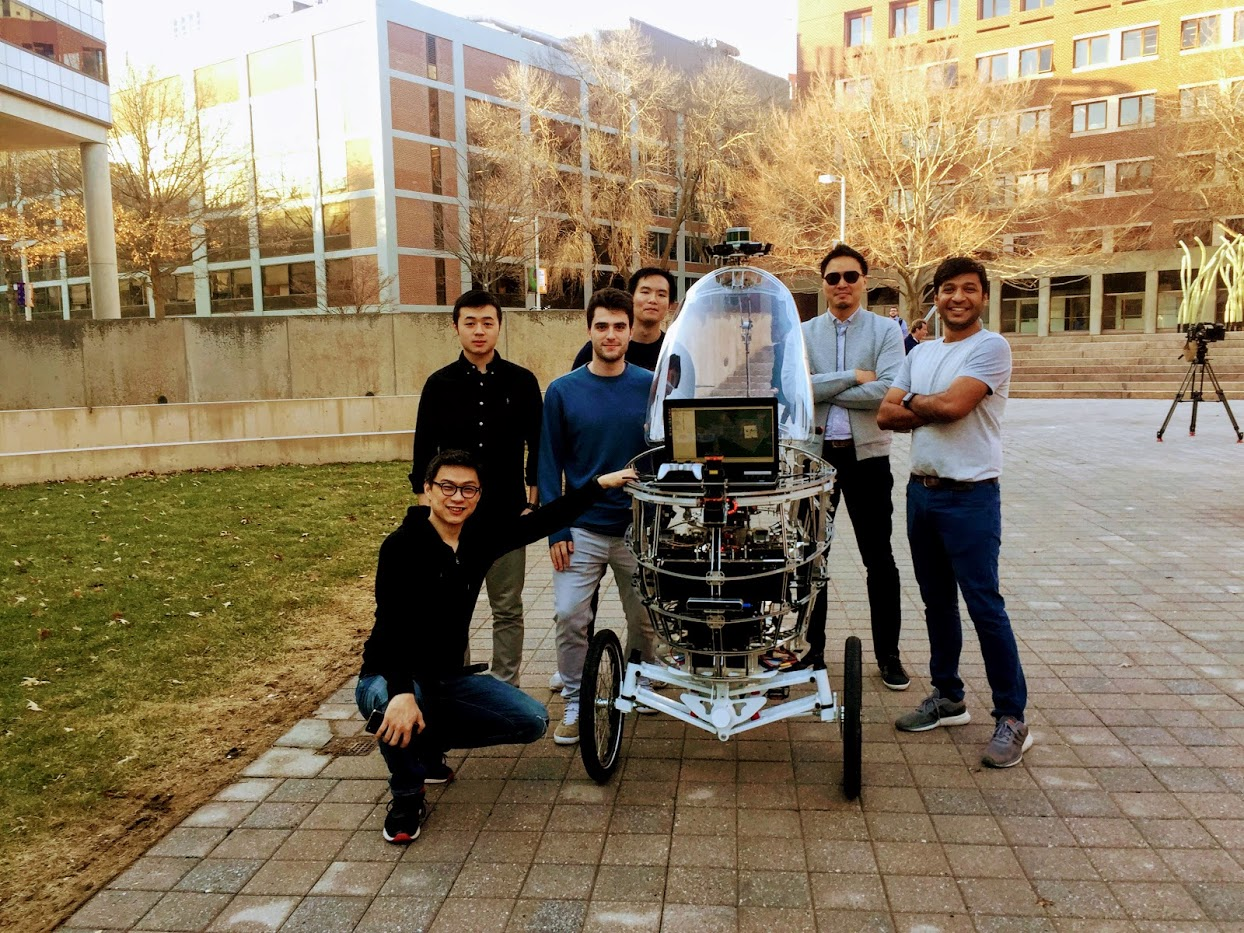
\includegraphics[width=.7\linewidth]{pictures/team}}
  \caption[The power of a team]{Alone we can do so little, together we can do so much}
\end{figure}